\section{Date: 2026-09-12}
\noindent \textbf{Series ID: CUUSA200SAH1} 

\noindent This series is titled Consumer Price Index for All Urban Consumers: Shelter in Midwest - Size Class A and has a frequency of Semiannual. The units are Index 1982-1984=100 and the seasonal adjustment is Not Seasonally Adjusted.The observation start date is 1984-01-01 and the observation end date is 2026-01-01.The popularity of this series is 1. \\ 

\noindent \textbf{Series ID: APU0400706111} 

\noindent This series is titled Average Price: Chicken, Fresh, Whole (Cost per Pound/453.6 Grams) in the West Census Region - Urban and has a frequency of Monthly. The units are U.S. Dollars and the seasonal adjustment is Not Seasonally Adjusted.The observation start date is 1980-01-01 and the observation end date is 2026-08-01.The popularity of this series is 14. \\ 

\subsection{Raw Regression}
\noindent Regresses the two series against each other directly. A significant result here can come just as easily from both series sharing a long-run trend as from any real relationship.

\begin{center}
\begin{tabular}{lclc}
\toprule
\textbf{Dep. Variable:}            & value\_fred\_APU0400706111 & \textbf{  R-squared:         } &     0.938   \\
\textbf{Model:}                    &            OLS             & \textbf{  Adj. R-squared:    } &     0.937   \\
\textbf{Method:}                   &       Least Squares        & \textbf{  F-statistic:       } &     1248.   \\
\textbf{Date:}                     &      Sat, 12 Sep 2026      & \textbf{  Prob (F-statistic):} &  8.79e-52   \\
\textbf{Time:}                     &          14:28:28          & \textbf{  Log-Likelihood:    } &    79.771   \\
\textbf{No. Observations:}         &               85           & \textbf{  AIC:               } &    -155.5   \\
\textbf{Df Residuals:}             &               83           & \textbf{  BIC:               } &    -150.7   \\
\textbf{Df Model:}                 &                1           & \textbf{                     } &             \\
\textbf{Covariance Type:}          &         nonrobust          & \textbf{                     } &             \\
\bottomrule
\end{tabular}
\begin{tabular}{lcccccc}
                                   & \textbf{coef} & \textbf{std err} & \textbf{t} & \textbf{P$> |$t$|$} & \textbf{[0.025} & \textbf{0.975]}  \\
\midrule
\textbf{const}                     &       0.1732  &        0.034     &     5.099  &         0.000        &        0.106    &        0.241     \\
\textbf{value\_fred\_CUUSA200SAH1} &       0.0053  &        0.000     &    35.326  &         0.000        &        0.005    &        0.006     \\
\bottomrule
\end{tabular}
\begin{tabular}{lclc}
\textbf{Omnibus:}       &  3.941 & \textbf{  Durbin-Watson:     } &    0.840  \\
\textbf{Prob(Omnibus):} &  0.139 & \textbf{  Jarque-Bera (JB):  } &    3.180  \\
\textbf{Skew:}          &  0.421 & \textbf{  Prob(JB):          } &    0.204  \\
\textbf{Kurtosis:}      &  3.436 & \textbf{  Cond. No.          } &     742.  \\
\bottomrule
\end{tabular}
%\caption{OLS Regression Results}
\end{center}

Notes: \newline
 [1] Standard Errors assume that the covariance matrix of the errors is correctly specified.

\begin{figure}
\centering
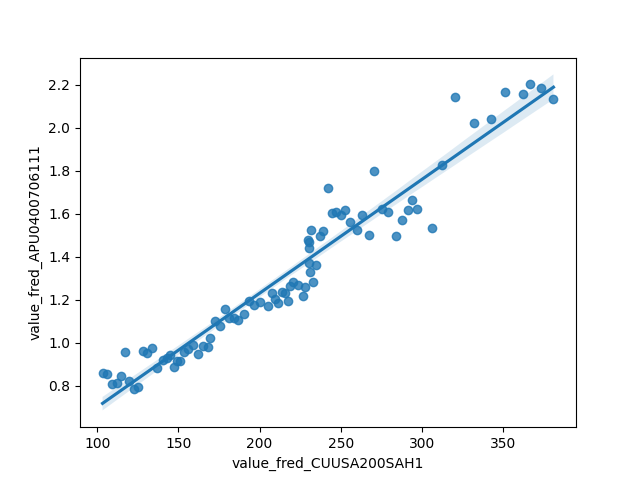
\includegraphics[scale = 0.9]{plots/plot_2026-09-12.png}
\caption{Raw Regression Plot for 2026-09-12}
\end{figure}
\newpage
\subsection{Detrended Regression}
\noindent Regresses the residuals of each series after removing its own linear time trend, so a shared trend can no longer drive the result on its own. A relationship that stays significant here is better evidence of a genuine link between the two series.

\begin{center}
\begin{tabular}{lclc}
\toprule
\textbf{Dep. Variable:}                       & value\_fred\_APU0400706111\_detrended & \textbf{  R-squared:         } &     0.370   \\
\textbf{Model:}                               &                  OLS                  & \textbf{  Adj. R-squared:    } &     0.363   \\
\textbf{Method:}                              &             Least Squares             & \textbf{  F-statistic:       } &     48.77   \\
\textbf{Date:}                                &            Sat, 12 Sep 2026           & \textbf{  Prob (F-statistic):} &  6.57e-10   \\
\textbf{Time:}                                &                14:28:28               & \textbf{  Log-Likelihood:    } &    79.794   \\
\textbf{No. Observations:}                    &                     85                & \textbf{  AIC:               } &    -155.6   \\
\textbf{Df Residuals:}                        &                     83                & \textbf{  BIC:               } &    -150.7   \\
\textbf{Df Model:}                            &                      1                & \textbf{                     } &             \\
\textbf{Covariance Type:}                     &               nonrobust               & \textbf{                     } &             \\
\bottomrule
\end{tabular}
\begin{tabular}{lcccccc}
                                              & \textbf{coef} & \textbf{std err} & \textbf{t} & \textbf{P$> |$t$|$} & \textbf{[0.025} & \textbf{0.975]}  \\
\midrule
\textbf{const}                                &    2.172e-14  &        0.010     &  2.09e-12  &         1.000        &       -0.021    &        0.021     \\
\textbf{value\_fred\_CUUSA200SAH1\_detrended} &       0.0055  &        0.001     &     6.984  &         0.000        &        0.004    &        0.007     \\
\bottomrule
\end{tabular}
\begin{tabular}{lclc}
\textbf{Omnibus:}       &  4.280 & \textbf{  Durbin-Watson:     } &    0.842  \\
\textbf{Prob(Omnibus):} &  0.118 & \textbf{  Jarque-Bera (JB):  } &    3.513  \\
\textbf{Skew:}          &  0.442 & \textbf{  Prob(JB):          } &    0.173  \\
\textbf{Kurtosis:}      &  3.459 & \textbf{  Cond. No.          } &     13.3  \\
\bottomrule
\end{tabular}
%\caption{OLS Regression Results}
\end{center}

Notes: \newline
 [1] Standard Errors assume that the covariance matrix of the errors is correctly specified.

\begin{figure}
\centering
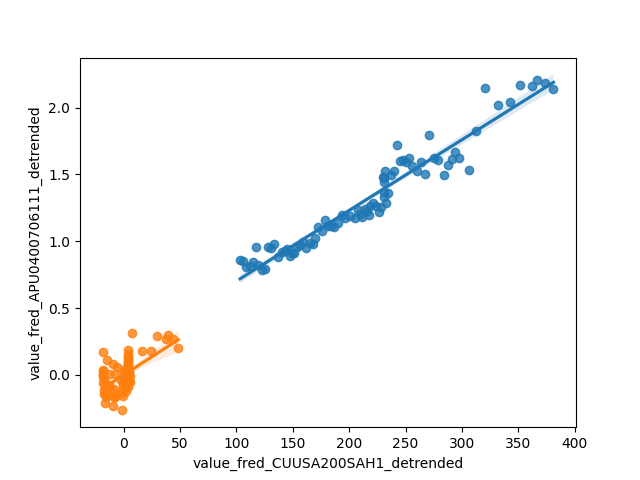
\includegraphics[scale = 0.9]{plots/plot_2026-09-12_detrended.png}
\caption{Detrended Regression Plot for 2026-09-12}
\end{figure}
\newpage
